\documentclass{beamer}
%\usepackage[orientation=portrait,size=custom,width=8,height=4,scale=0.3,debug]{beamerposter} 

\RequirePackage{natbib}
\setcitestyle{authoryear,round,citesep={;},aysep={,},yysep={;}}

\mode<presentation>
{
  \usetheme{default}
  \usecolortheme{default}
  \usefonttheme{professionalfonts}
  \setbeamertemplate{navigation symbols}{}
  \setbeamertemplate{caption}[numbered]
}

\usepackage[english]{babel}
\usepackage[utf8]{inputenc}

\usepackage{amsmath}
\usepackage{amsfonts}
\usepackage{amsthm}
\usepackage{bibentry}
\usepackage{graphicx}
\usepackage{bm}
\usepackage{booktabs}
\usepackage{tikz}
\usepackage{xcolor}
\usepackage{multirow}
\usepackage[normalem]{ulem}
\usepackage{pifont}
\usepackage{array}
\usepackage{multimedia}
\usepackage{makecell}
\usepackage{xspace}
\usepackage{CJKutf8}
\usepackage{pdfpages}


\renewcommand{\ULthickness}{1.2pt}
\graphicspath{{figures/}}

\DeclareMathOperator*{\argmin}{\arg\!\min}
\DeclareMathOperator*{\argmax}{\arg\!\max}
\DeclareMathOperator*{\substr}{substr}
\DeclareMathOperator*{\subseq}{subseq}
\DeclareMathOperator*{\len}{len}

\newcommand{\SubItem}[1]{
    {\setlength\itemindent{15pt} \item[-] #1}
}

\definecolor{color0}{HTML}{FFFFFF}
\definecolor{color1}{HTML}{FEE5D8}
\definecolor{color2}{HTML}{FDCAB5}
\definecolor{color3}{HTML}{FCAB8F}
\definecolor{color4}{HTML}{FC8A6A}
\definecolor{color5}{HTML}{FB694A}
\definecolor{color6}{HTML}{F14432}
\definecolor{color7}{HTML}{D92523}
\definecolor{color8}{HTML}{BC141A}
\definecolor{color9}{HTML}{980C13}
\definecolor{color10}{HTML}{800080}
\definecolor{easy}{HTML}{02C386}
\definecolor{hard}{HTML}{C00202}
\newcommand*{\mybox}[2]{\tikz[anchor=base,baseline=0pt,rounded corners=0pt,inner sep=0.2mm] \node[fill=#1!60!white] (X) {#2};}
\newcommand*{\mybbox}[2]{\tikz[anchor=base,baseline=0pt,inner sep=0.2mm,] \node[draw=black,thick,fill=#1!60!white] (X) {#2};}


\definecolor{l10_color1}{HTML}{3232FF}
\definecolor{coloranswer}{HTML}{0596FF}
\definecolor{lightblue}{HTML}{3CC7EA}
\definecolor{boxcolor}{HTML}{EEEEEE}
\definecolor{periwinkle}{rgb}{0.8, 0.8, 1.0}
\definecolor{colorsquad}{rgb}{0,1,0}
\definecolor{colorsnli}{rgb}{1,0,0}
\definecolor{colorvqa}{rgb}{1,1,0}

\newcommand\BibTeX{B{\sc ib}\TeX}
\newcommand{\abr}[1]{\textsc{#1}}
\newcommand{\nlp}{\textsc{nlp}}
\newcommand{\mb}[1]{\boldsymbol{\mathbf{#1}}}
\newcommand{\g}{\, | \,}
\newcommand{\mtanchor}{MTAnchor\xspace}
\newcommand{\zh}[2][]{\begin{CJK*}{UTF8}{bsmi}{#1}{#2}\end{CJK*}}


\newcommand*\colourcheck[1]{%
  \expandafter\newcommand\csname #1check\endcsname{\textcolor{#1}{\ding{52}}}%
}
\colourcheck{blue}

\title{Multilingual Anchoring: Interactive Topic Modeling and Alignment across Languages}
\author{
\small{
\textbf{Michelle Yuan}$^1$ Benjamin Van Durme$^2$  Jordan Boyd-Graber$^1$
} \\\vspace{10px}
\footnotesize{$^1$University of Maryland $^2$John Hopkins University}
}
\date{}

\begin{document}



\begin{frame}
    \titlepage
\end{frame}

% authors
\begin{frame}[c]{Authors}
\begin{center}
\begin{tabular}{ccc}
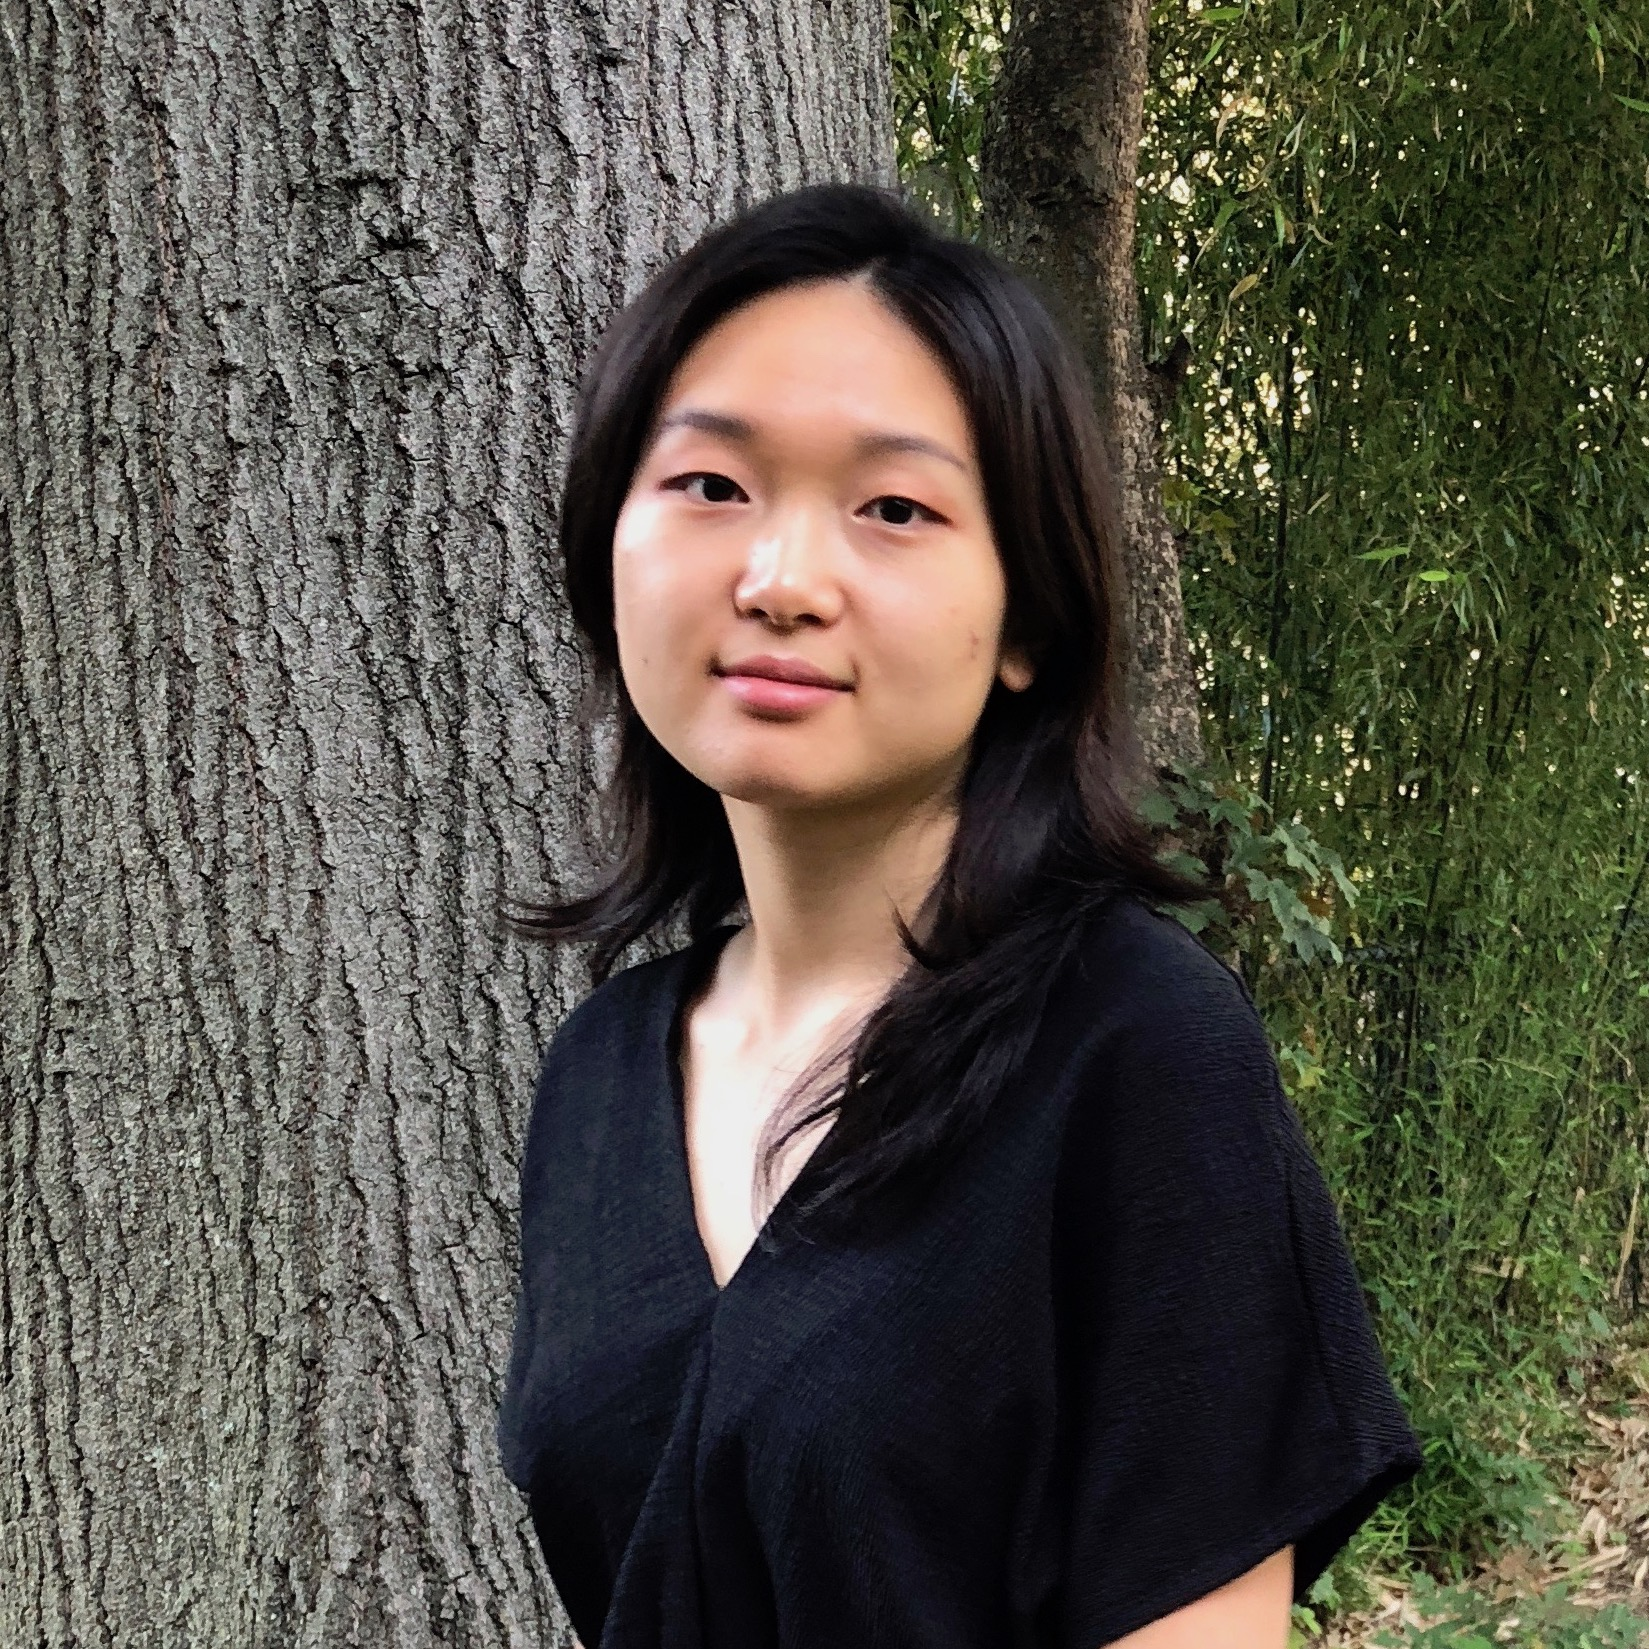
\includegraphics[width=.25\linewidth]{michelle}   & 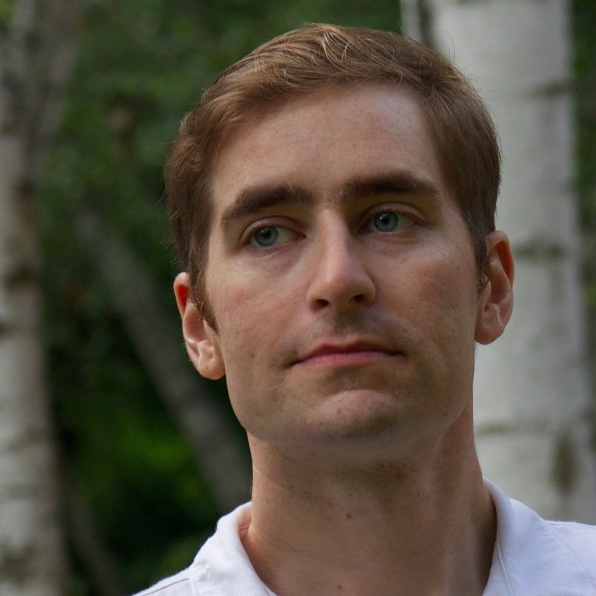
\includegraphics[width=.25\linewidth]{ben}  & 
\includegraphics[width=.25\linewidth]{jordan} \\
    Michelle Yuan & Benjamin Van Durme & Jordan Boyd-Graber \\
    UMD & JHU & UMD \\
\end{tabular}
\end{center}
\end{frame}




% 1. multilingual topic modeling
\begin{frame}
\begin{itemize}
\item Large text collections often require topic triage quickly in low-resource settings (e.g. natural disaster, political instability). \pause
\item Analysts need to examine multilingual text collections, but are scarce in one or more languages.
\end{itemize}
\end{frame}

\begin{frame}{Modeling Multilingual Topics}
\begin{figure}
\begin{center}
\begin{overprint}
\onslide<1>\centerline{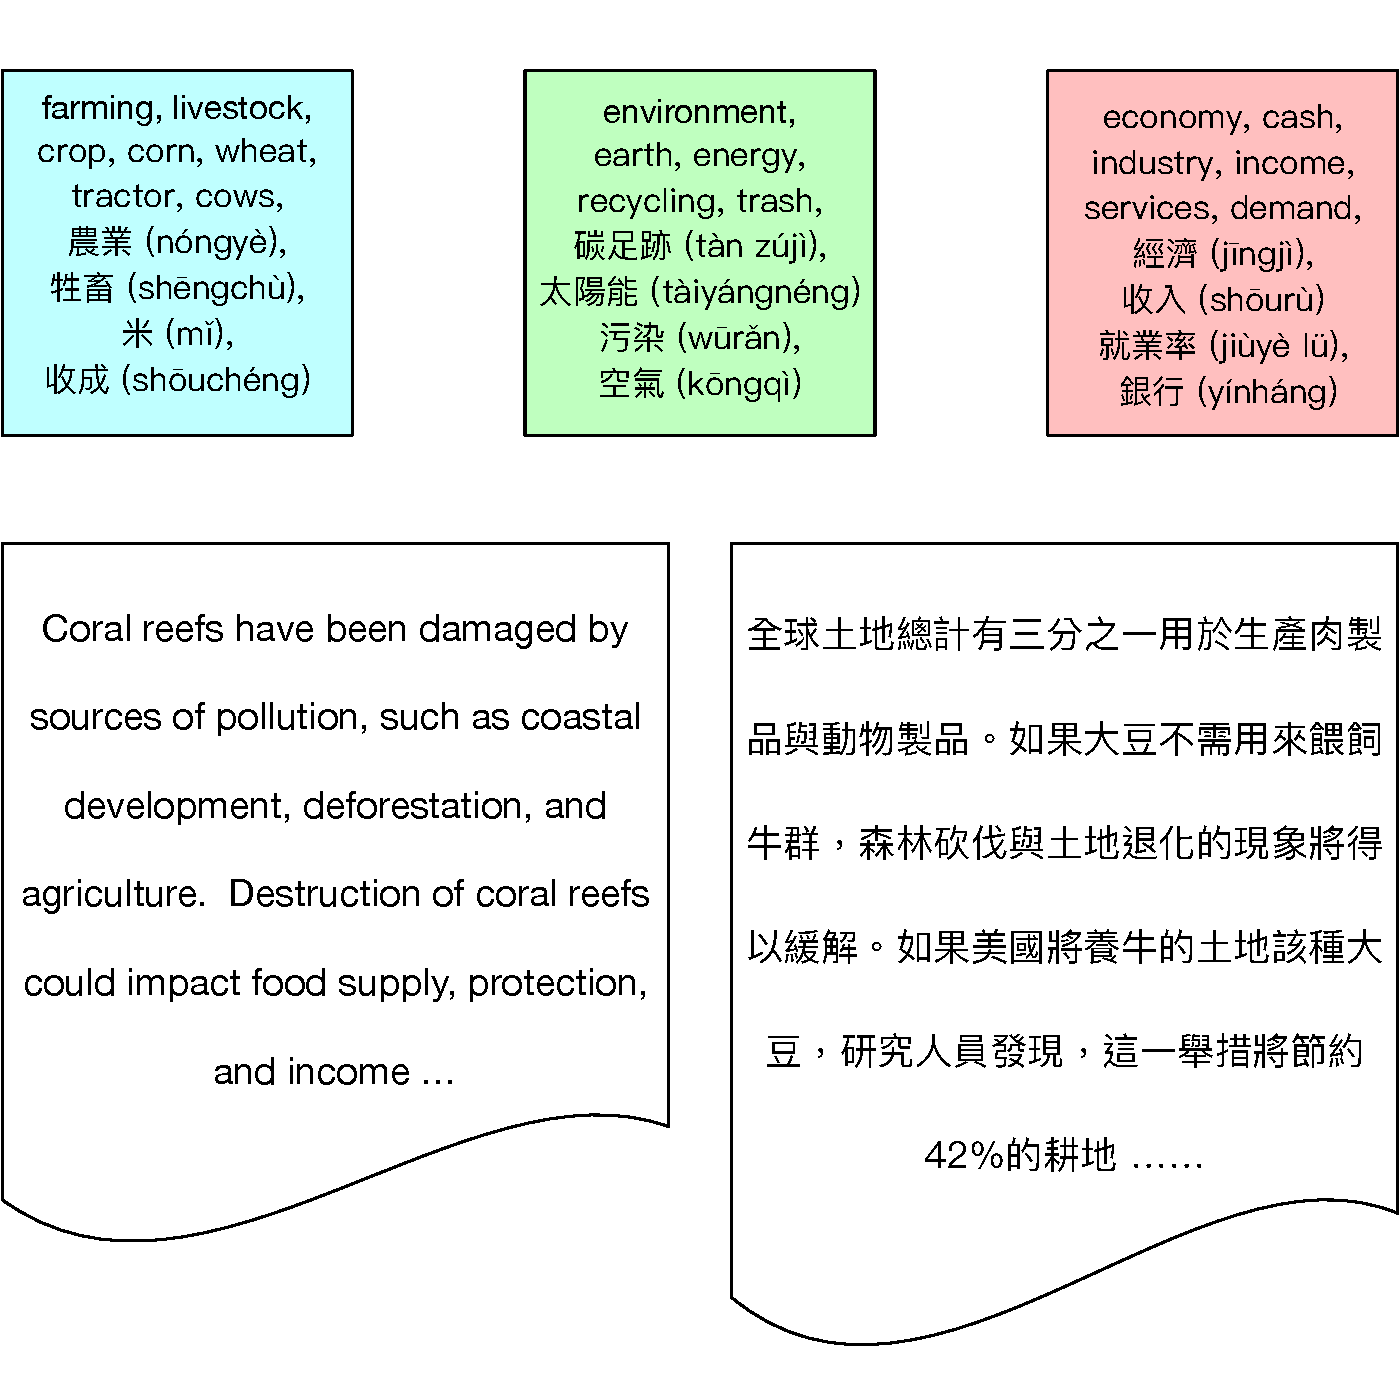
\includegraphics[width=0.7\textwidth]{articles1.pdf}}
\onslide<2>\centerline{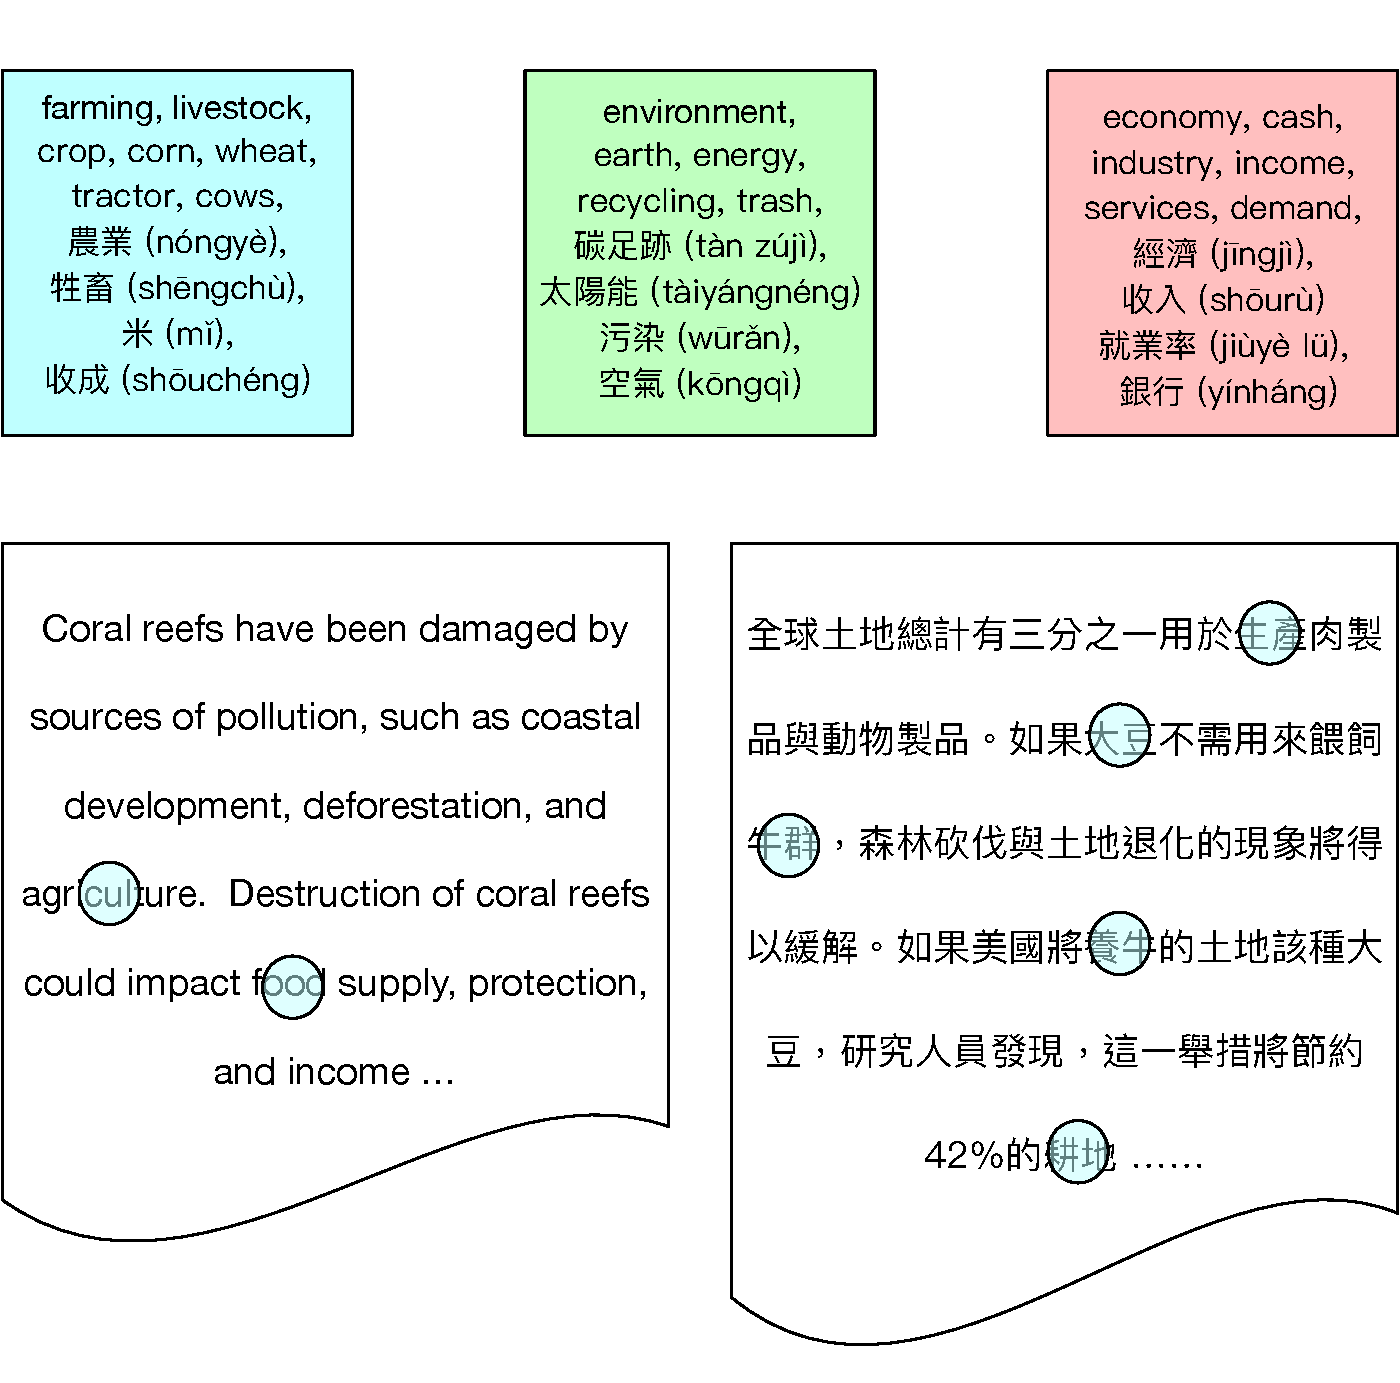
\includegraphics[width=0.7\textwidth]{articles2.pdf}}
\onslide<3>\centerline{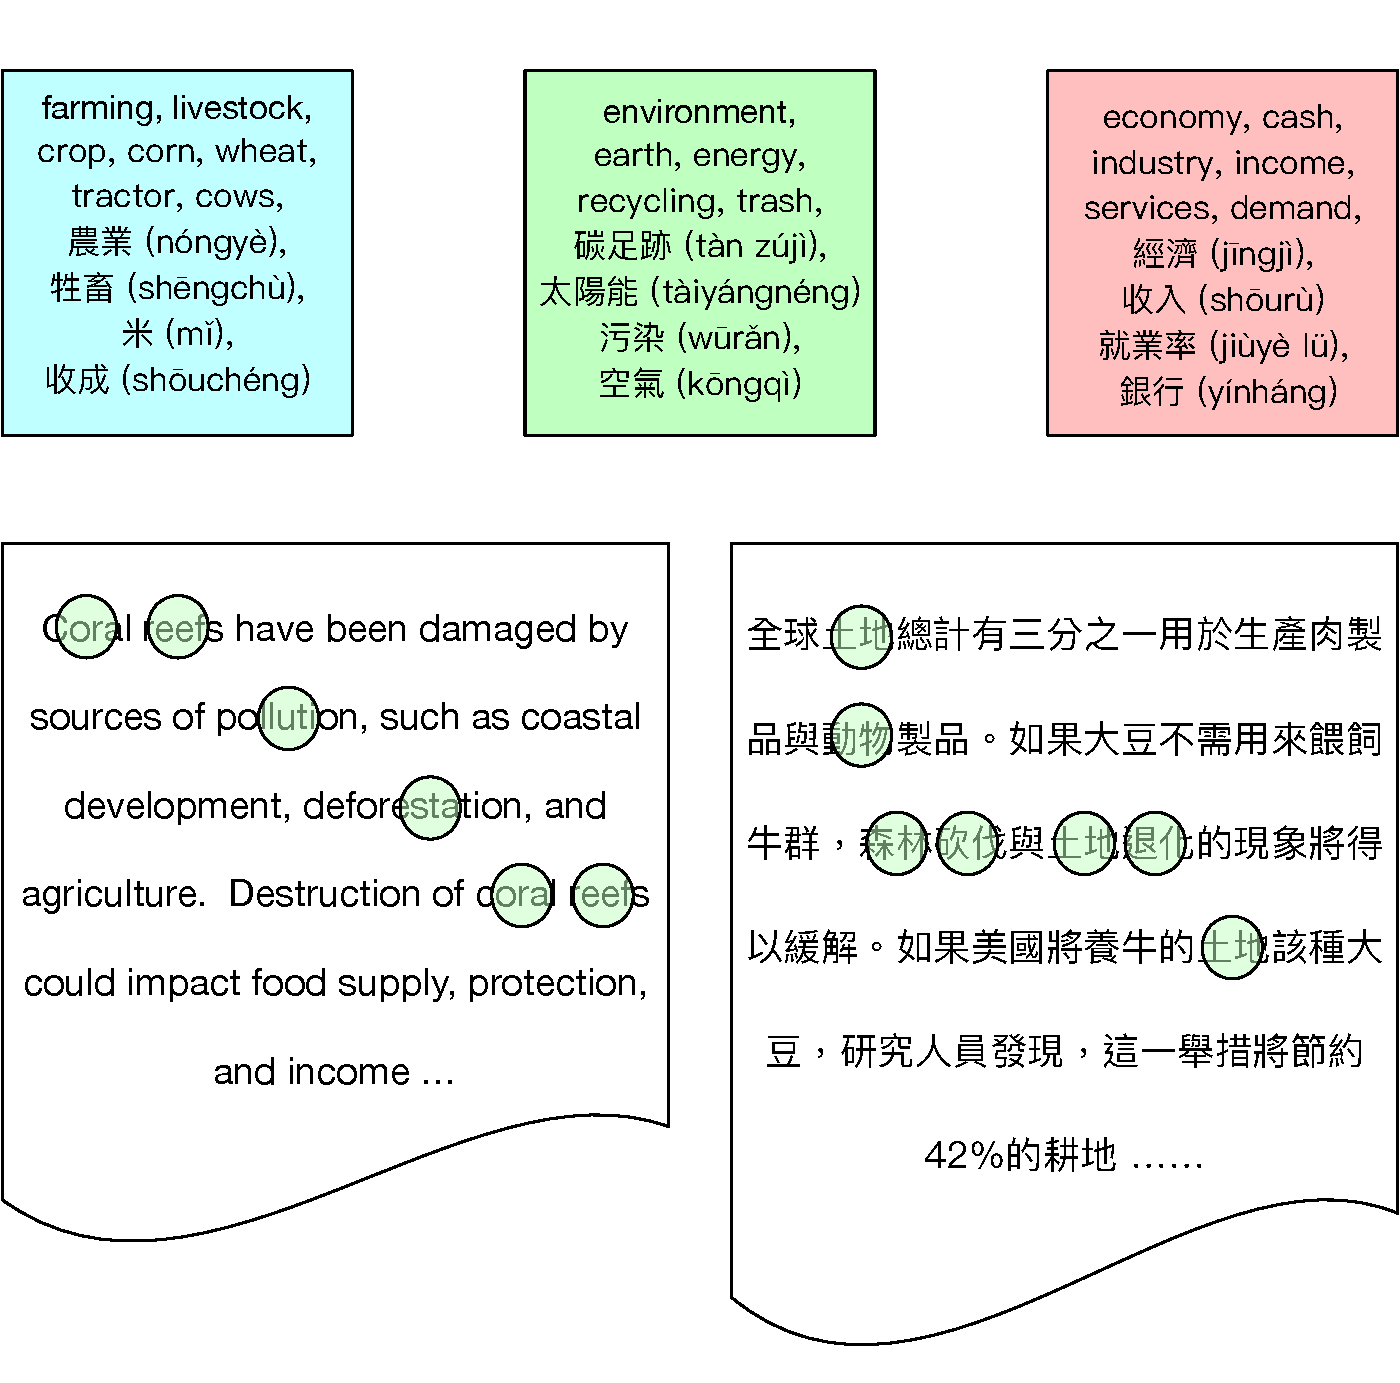
\includegraphics[width=0.7\textwidth]{articles3.pdf}}
\onslide<4>\centerline{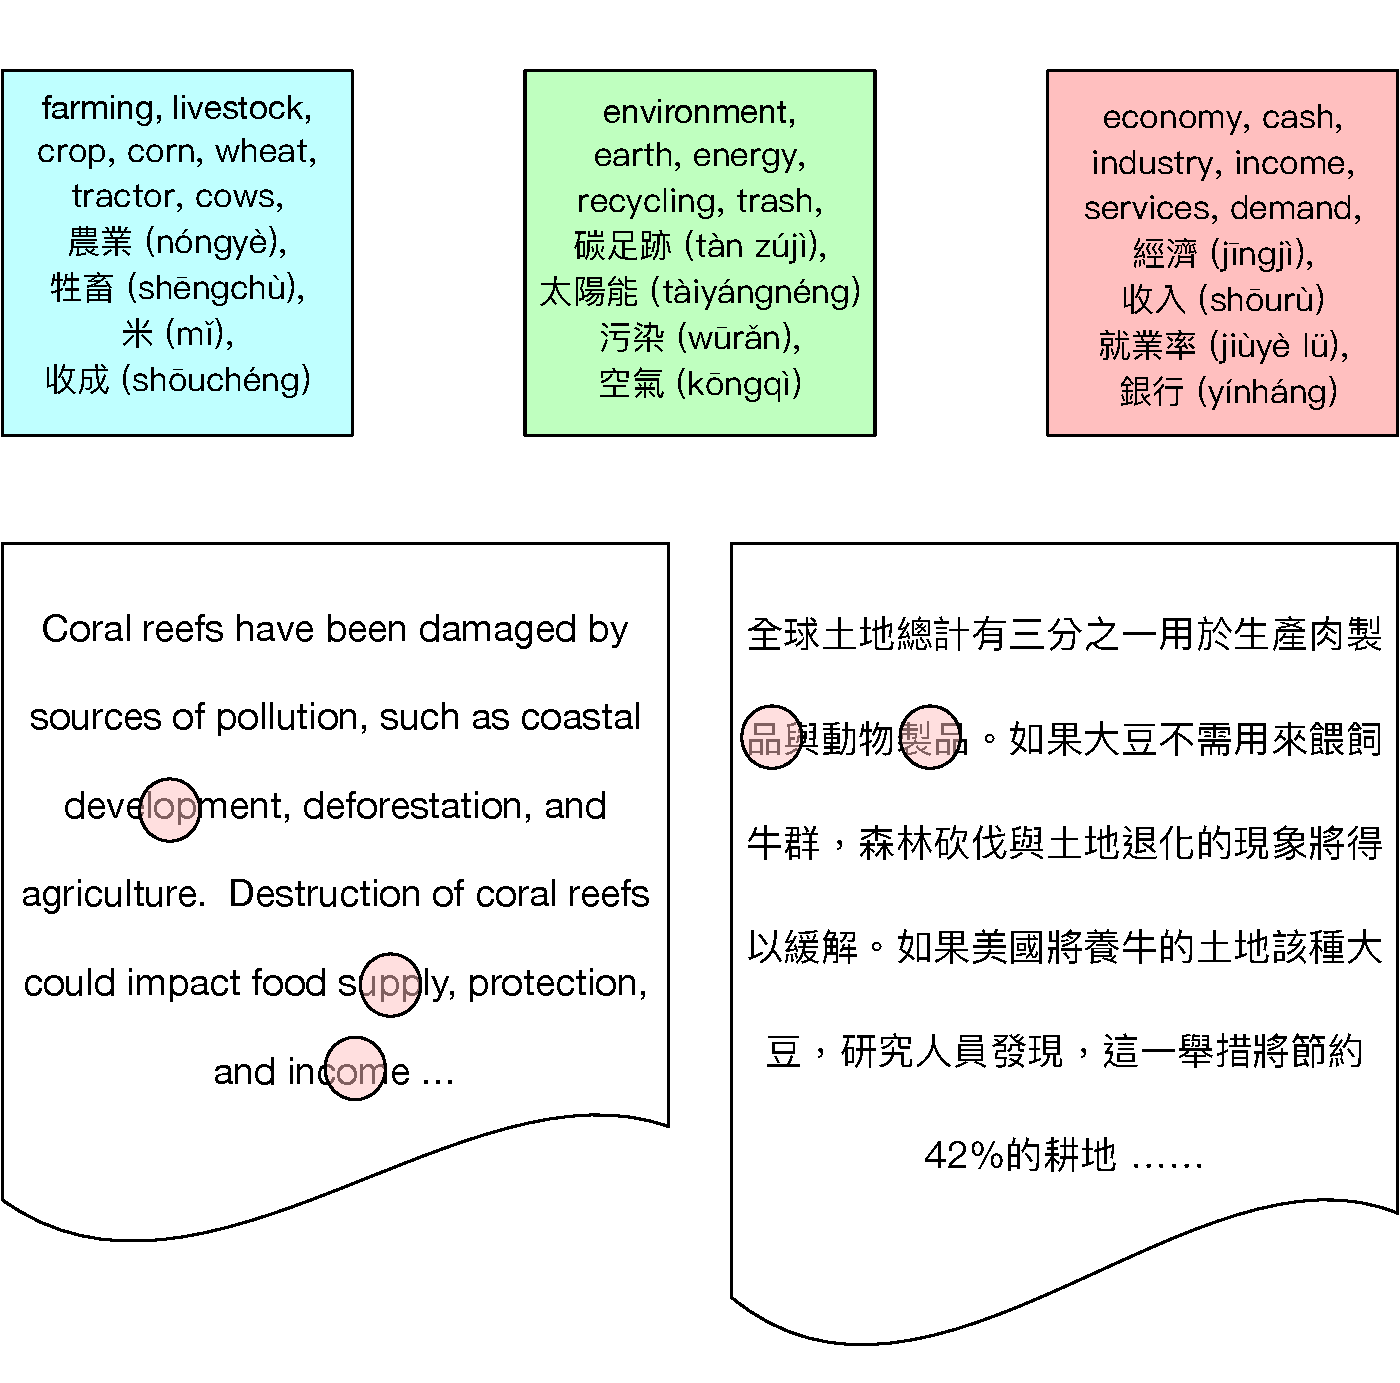
\includegraphics[width=0.7\textwidth]{articles4.pdf}}
\onslide<5->\centerline{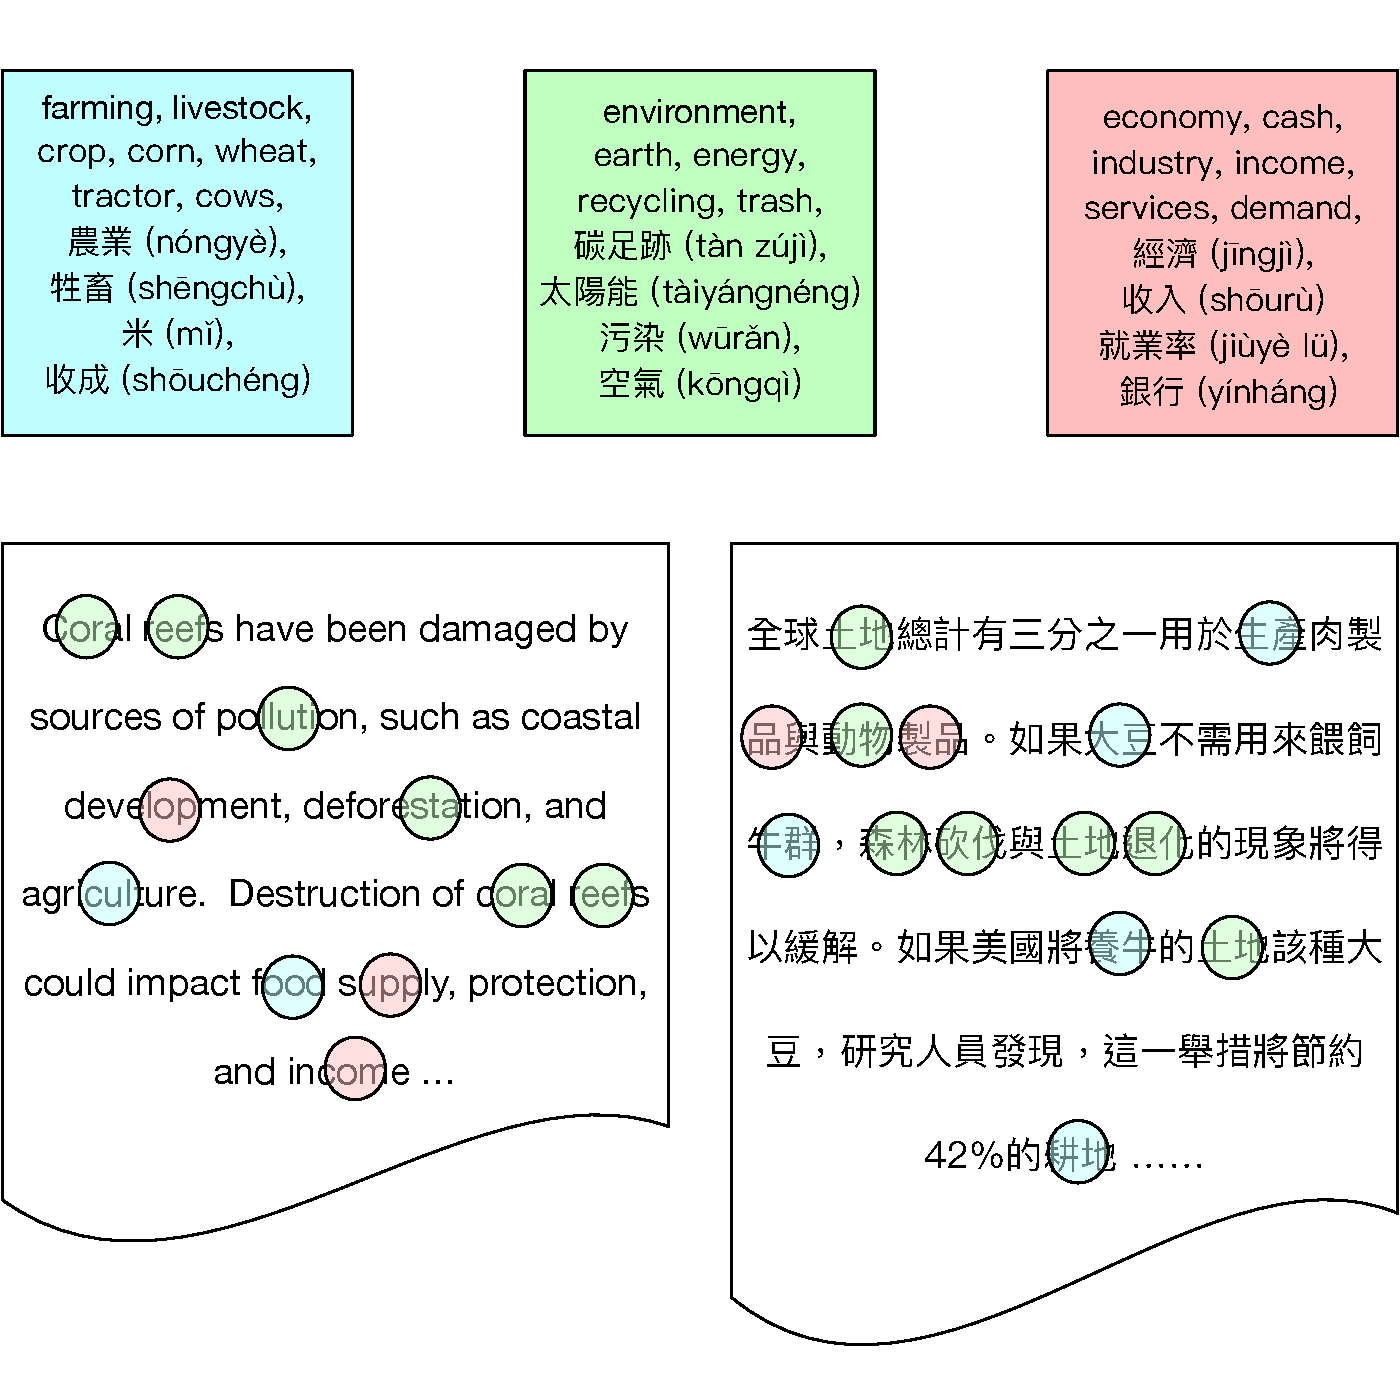
\includegraphics[width=0.7\textwidth]{articles5.pdf}}
\end{overprint}
\end{center}
\end{figure}
\end{frame}

\begin{frame}{Generative Approaches}
\begin{itemize}
\item Polylingual Topic Model~\citep{mimno-2009}
\item Joint\abr{lda}~\citep{jagarlamudi-2010}
\item Polylingual Tree-based Topic model~\citep{hu-2014-ptlda} 
\item \abr{mcta}~\citep{shi-2016} \pause
\vspace{1cm}
\end{itemize}
\textbf{These methods are slow, assume extensive knowledge about languages, and preclude human refinement.}
\end{frame}



% 2. anchoring
% active learning
\begin{frame}{Method: Active Learning}
    \begin{itemize}
        \item<1-> Use active learning to find particular spans of text for users to label
    %\centerline{\includegraphics[width=\textwidth]{\figfile{example_target.pdf}}}
        \item<2-> The goal is to adapt the model to the target domain by continue
training it on spans labeled from active learning
    \end{itemize}
\end{frame}


\begin{frame}{What should we label?}
    \onslide<1->
       \begin{quote}
           A fantastic \spot<2>[fill=green]{experience}, very informative, very
           \spot<2>[fill=green]{time} consuming but enjoyable. So much information to take
           in about Guinness that \spot<4>[fill=red]{you} would’ve never known. For
           example, \spot<3>[fill=Orchid]{the brewery} hired the statistician Willam Gosset
           in 1899. \spot<3>[fill=Orchid]{The “student”} was known for developing
           the Student’s t-test,
           \spot<5>[fill=SkyBlue]{a well-known method in statistical
           inference}.
       \end{quote}
       \centering
       \medskip
    \only<2>{\textcolor{green}{Uncertainty in mention detection}}
    \only<3>{\textcolor{Orchid}{Uncertainty in mention clustering}}
    \only<4>{\textcolor{red}{Uncertainty in mention clustering
    conditioned on mention detection}}
    \only<5>{\textcolor{SkyBlue}{Uncertainty in both mention detection
    and mention clustering}}
\end{frame}

%\begin{frame}{Method: Active Learning}
%We explore active learning for adapting CR models by:
%\begin{enumerate}
%\onslide<1-> \item Sampling spans according to different sources of model
%uncertainty
%\onslide<2-> \item Understanding the trade-off between reading and labeling
%costs
%\end{enumerate}
%\end{frame}


% % % 3. multilingual anchoring/mtanchor
\begin{frame}{Let's Take a Step Back}
\begin{table}
\centering
\begin{tabular}{cc}
Model Overconfidence & Rubbish Examples \\
\cite{guo2017calibration} & \cite{goodfellow2014explaining} \\
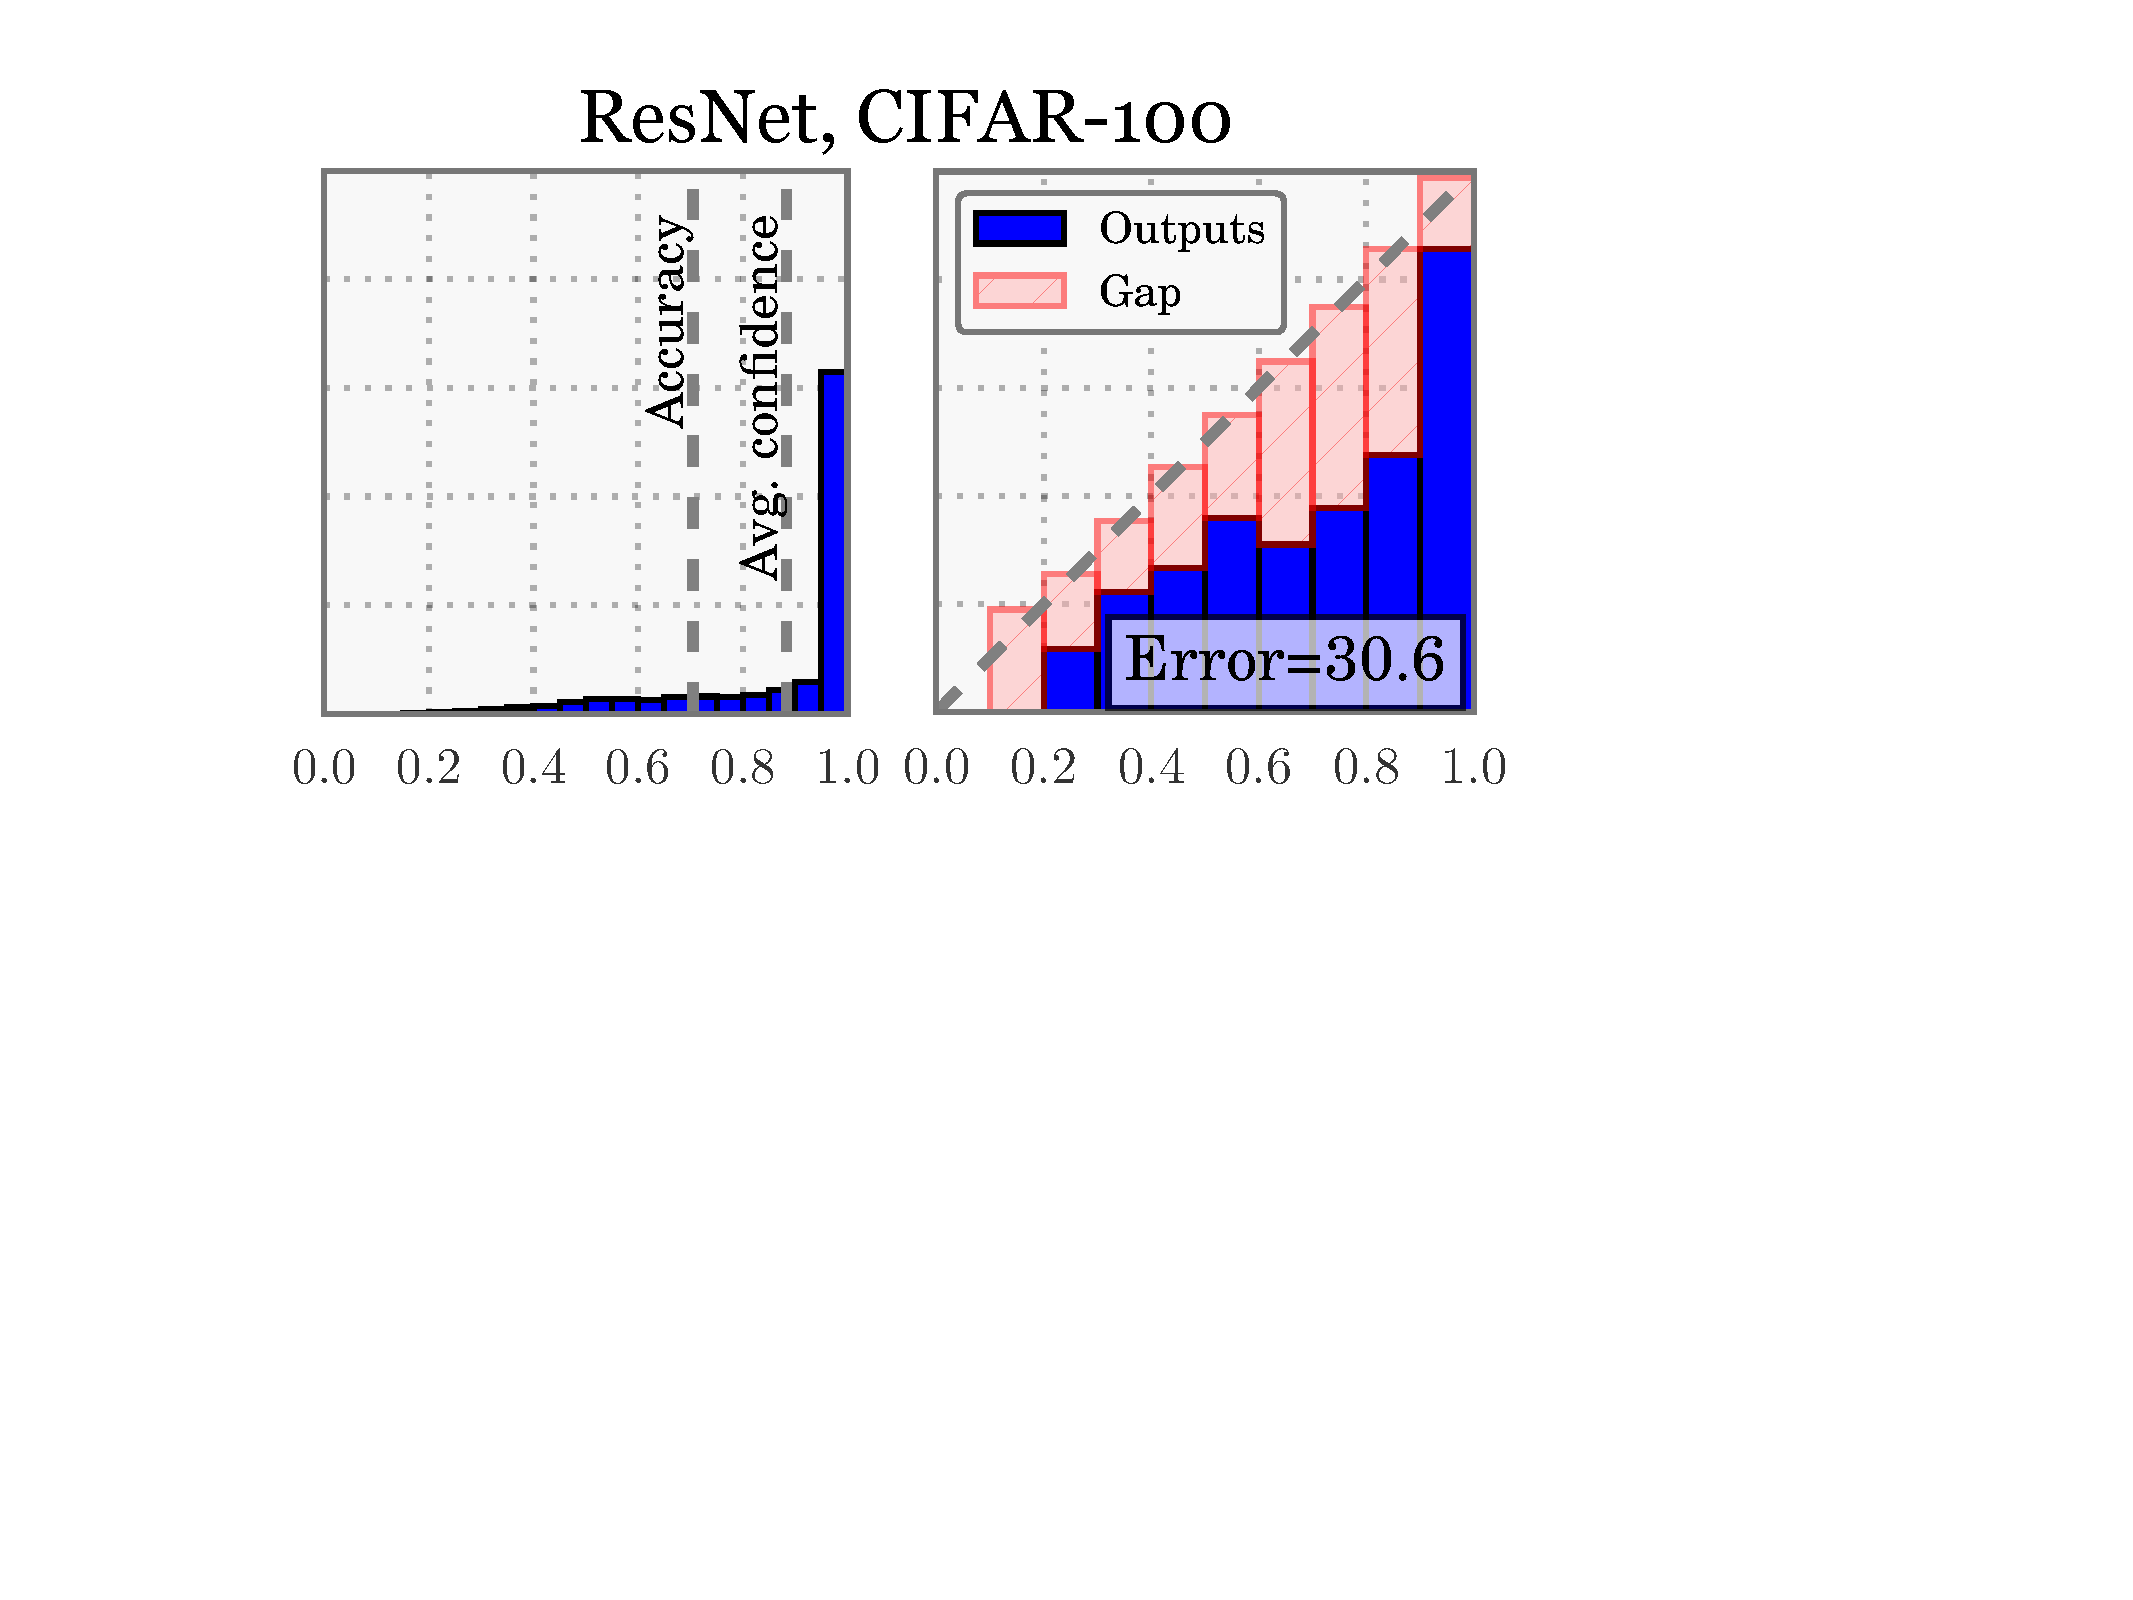
\includegraphics[height=2.5cm]{guo} & 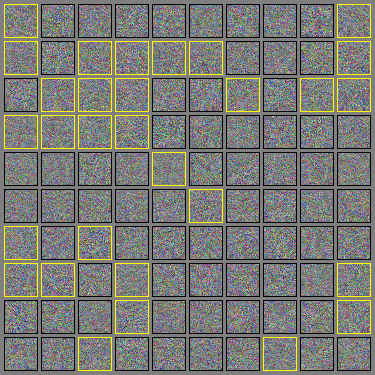
\includegraphics[height=2.5cm]{rubbish} 
\end{tabular}
\end{table}
\begin{itemize}
\pause
% \item Overconfidence alone does not fully explain why confidence is high
% on these non-sensical inputs. \pause
\item Overconfidence does not cover non-sensical inputs. \pause
\item Reduced examples are rubbish examples. \pause
\item \textbf{How did input reduction lead to rubbish examples?}
\end{itemize}
\end{frame}

\begin{frame}{Issues of Linear, Confidence-based Interpretation}
\begin{table}
\small
\begin{tabular}{p{0.72\columnwidth}l}
\textbf{\squad{}}  \\
\multicolumn{2}{p{0.9\columnwidth}}{The Panthers used the San Jose State practice facility and
stayed at the San Jose Marriott. The Broncos practiced at
\mybox{coloranswer}{Stanford University} and stayed at the Santa Clara
Marriott.} \\\\
Question & Confidence \\\midrule
Where did the {Broncos} practice for the Super Bowl ? & (0.90, 0.89) \pause\\
Where did the \textcolor{white}{Broncos} practice for the Super Bowl ? & (0.92, 0.88) \\
\end{tabular}
\end{table}
\begin{itemize}
\pause
\item Confidence remains high after the crucial word is removed.
\pause
\item Decrease in confidence does not align with importance.
\pause
\item After the first reduction step, the input is already rubbish.
\end{itemize}
\end{frame}

\begin{frame}{Issues of Linear, Confidence-based Interpretation}
\textbf{\squad{}} \\
QuickBooks sponsored a ``Small Business Big Game'' contest, in
which Death Wish Coffee had a 30-second commercial aired free of
charge courtesy of QuickBooks. \mybox{coloranswer}{Death Wish
Coffee} beat out nine other contenders from across the United
States for the free advertisement. \newline \newline
%  \mybox{color1}{\strut{What}} \mybox{color1}{\strut{company}} \mybox{color1}{\strut{won}} \mybox{color1}{\strut{free}} \mybox{color6}{\strut{advertisement}} \mybox{color1}{\strut{due}} \mybox{color1}{\strut{to}} \mybox{color1}{\strut{QuickBooks}} \mybox{color0}{\strut{\underline{contest}}} \mybox{color1}{\strut{?}}\\
 \mybox{color1}{\strut{What}} \mybox{color1}{\strut{company}} \mybox{color1}{\strut{won}} \mybox{color1}{\strut{free}} \mybox{color6}{\strut{advertisement}} \mybox{color1}{\strut{due}} \mybox{color1}{\strut{to}} \mybox{color0}{\strut{\underline{QuickBooks}}} \mybox{color1}{\strut{?}}\\
 \mybox{color2}{\strut{What}} \mybox{color0}{\strut{company}} \mybox{color1}{\strut{won}} \mybox{color1}{\strut{free}} \mybox{color0}{\strut{\underline{advertisement}}} \mybox{color1}{\strut{due}} \mybox{color1}{\strut{to}} \mybox{color5}{\strut{?}}\\
 \mybox{color1}{\strut{What}} \mybox{color0}{\strut{\underline{company}}} \mybox{color1}{\strut{won}} \mybox{color1}{\strut{free}} \mybox{color1}{\strut{due}} \mybox{color1}{\strut{to}} \mybox{color5}{\strut{?}}\\
 \mybox{color1}{\strut{What}} \mybox{color4}{\strut{won}} \mybox{color0}{\strut{\underline{free}}} \mybox{color1}{\strut{due}} \mybox{color0}{\strut{to}} \mybox{color5}{\strut{?}}\\
 \mybox{color1}{\strut{What}} \mybox{color1}{\strut{won}} \mybox{color1}{\strut{due}} \mybox{color1}{\strut{to}} \mybox{color0}{\strut{\underline{?}}}\\
 \mybox{color1}{\strut{What}} \mybox{color4}{\strut{won}} \mybox{color1}{\strut{due}} \mybox{color0}{\strut{\underline{to}}}\\
 \mybox{color4}{\strut{What}} \mybox{color2}{\strut{won}} \mybox{color1}{\strut{\underline{due}}}\\
 \mybox{color2}{\strut{What}} \mybox{color1}{\strut{\underline{won}}}\\
 \mybox{color2}{\strut{What}}\\

\small
\mybox{color1}{\strut{What}} \mybox{color1}{\strut{company}}
\mybox{color1}{\strut{won}} \mybox{color1}{\strut{free}}
\mybox{color6}{\strut{advertisement}} \mybox{color1}{\strut{due}}
\mybox{color1}{\strut{to}} \mybox{color1}{\strut{QuickBooks}}
\mybox{color0}{\strut{{contest}}} \mybox{color1}{\strut{?}}\\\pause

\mybox{color1}{\strut{What}} \mybox{color1}{\strut{company}}
\mybox{color1}{\strut{won}} \mybox{color1}{\strut{free}}
\mybox{color6}{\strut{advertisement}} \mybox{color1}{\strut{due}}
\mybox{color1}{\strut{to}} \mybox{color0}{\strut{{QuickBooks}}}
\mybox{color1}{\strut{?}}\\\pause

\mybox{color2}{\strut{What}} \mybox{color0}{\strut{company}}
\mybox{color1}{\strut{won}} \mybox{color1}{\strut{free}}
\mybox{color0}{\strut{{advertisement}}} \mybox{color1}{\strut{due}}
\mybox{color1}{\strut{to}} \mybox{color5}{\strut{?}}\\\pause

\mybox{color1}{\strut{What}} \mybox{color0}{\strut{{company}}}
\mybox{color1}{\strut{won}} \mybox{color1}{\strut{free}}
\mybox{color1}{\strut{due}} \mybox{color1}{\strut{to}}
\mybox{color5}{\strut{?}}\\

\mybox{color1}{\strut{What}} \mybox{color4}{\strut{won}}
\mybox{color0}{\strut{{free}}} \mybox{color1}{\strut{due}}
\mybox{color0}{\strut{to}} \mybox{color5}{\strut{?}}\\

% \mybox{color1}{\strut{What}} \mybox{color1}{\strut{won}}
% \mybox{color1}{\strut{due}} \mybox{color1}{\strut{to}}
% \mybox{color0}{\strut{{?}}}\\
% 
% \mybox{color1}{\strut{What}} \mybox{color4}{\strut{won}}
% \mybox{color1}{\strut{due}} \mybox{color0}{\strut{{to}}}\\
% 
% \mybox{color4}{\strut{What}} \mybox{color2}{\strut{won}}
% \mybox{color1}{\strut{{due}}}\\
% 
% \mybox{color2}{\strut{What}} \mybox{color1}{\strut{{won}}}\\
% \mybox{color2}{\strut{What}}\\
\pause
\begin{itemize}
\item Independent word importance implicitly assumes bag-of-words.
\item Higher-order correlations are ignored.
\end{itemize}
\end{frame}

% % % 4. experiments/results
\begin{frame}{Task}
\onslide<1-> Document classification for detecting medical emergencies in low-resource languages\\\
\onslide<2-> \begin{table}[t]
    \centering
    \begin{tabular}{p{0.1\textwidth}p{0.8\textwidth}}
    \toprule
    %\textbf{English} &
    %... Seven inmates from the Bureau of Jail Management and Penology (BJMP),
    %Laoag City, have been transferred to the isolation room due to chicken
    %pox ...\\
	%\midrule
	\textbf{Ilocano} &
    ... Nagtalinaed dagiti pito a balod ti Bureau of Jail Management and
    Penology (BJMP) ditoy ciudad ti Laoag iti isolation room gapo iti tuko ...\\
    \bottomrule
  \end{tabular}
\end{table}
\end{frame}

\begin{frame}{Experiments}
\begin{itemize}
    \item \textbf{Embeddings:} fastText~\citep{bojanowski-17} aligned with
        \abr{rcsls}~\citep{joulin-2017}
\item \textbf{Classifier:} \abr{cnn} (max-pooling)
\item \textbf{Source language:} English
\item \textbf{Target language:} Ilocano
\end{itemize}
\end{frame}

\begin{frame}{User Study}
\begin{figure}
\centering
\includegraphics[width=0.8\textwidth]{\figfile{ui-il.png}}
\end{figure}
\end{frame}

\begin{frame}{Comparison}
\begin{itemize}
\item \textbf{Base:} original \abr{clwe} and original training dataset
\item \textbf{Active:} original \abr{clwe} and training dataset augmented by active learning
\item \textbf{CLIME:} refined \abr{clwe} and original training dataset
\item \textbf{A+C:} refined \abr{clwe} and training dataset augmented by active learning
\end{itemize}
\end{frame}

\begin{frame}{Results}
\begin{overprint}
\onslide<1>\centerline{\includegraphics[width=0.6\textwidth]{\figfile{acc1.png}}}
\onslide<2>\centerline{\includegraphics[width=0.6\textwidth]{\figfile{acc2.png}}}
\onslide<3>\centerline{\includegraphics[width=0.6\textwidth]{\figfile{acc3.png}}}
\onslide<4->\centerline{\includegraphics[width=0.6\textwidth]{\figfile{acc4.png}}}
\end{overprint}
\end{frame}

% % % 5. discussion/conclusion
% conclusion
\begin{frame}{Summary}
\begin{enumerate}
\item Neural CR models cannot immediately adapt without training on in-domain,
labeled data
\item To reduce amount of annotation, we use active learning to choose particular text spans for users to label
\item We explore various aspects of active learning for CR, including sources of
model uncertainty and the trade-off between reading and labeling
\item Sampling by mention detection entropy is more useful for domains like
PreCo
\item In both simulations and the user study,
CR improves from continued training on spans sampled from the same document rather than different
contexts
\end{enumerate}
\end{frame}



\begin{frame}[t, allowframebreaks]
\frametitle{References}
\bibliographystyle{../../style/emnlp2018}
\small
\bibliography{../../bib/journal-abbrv,../../bib/michelle,../../bib/jbg}
\end{frame}


\end{document}
